 

\section*{Aufgabe 1: \emph{Zwei Populationen}}


\begin{figure}
	\centering
	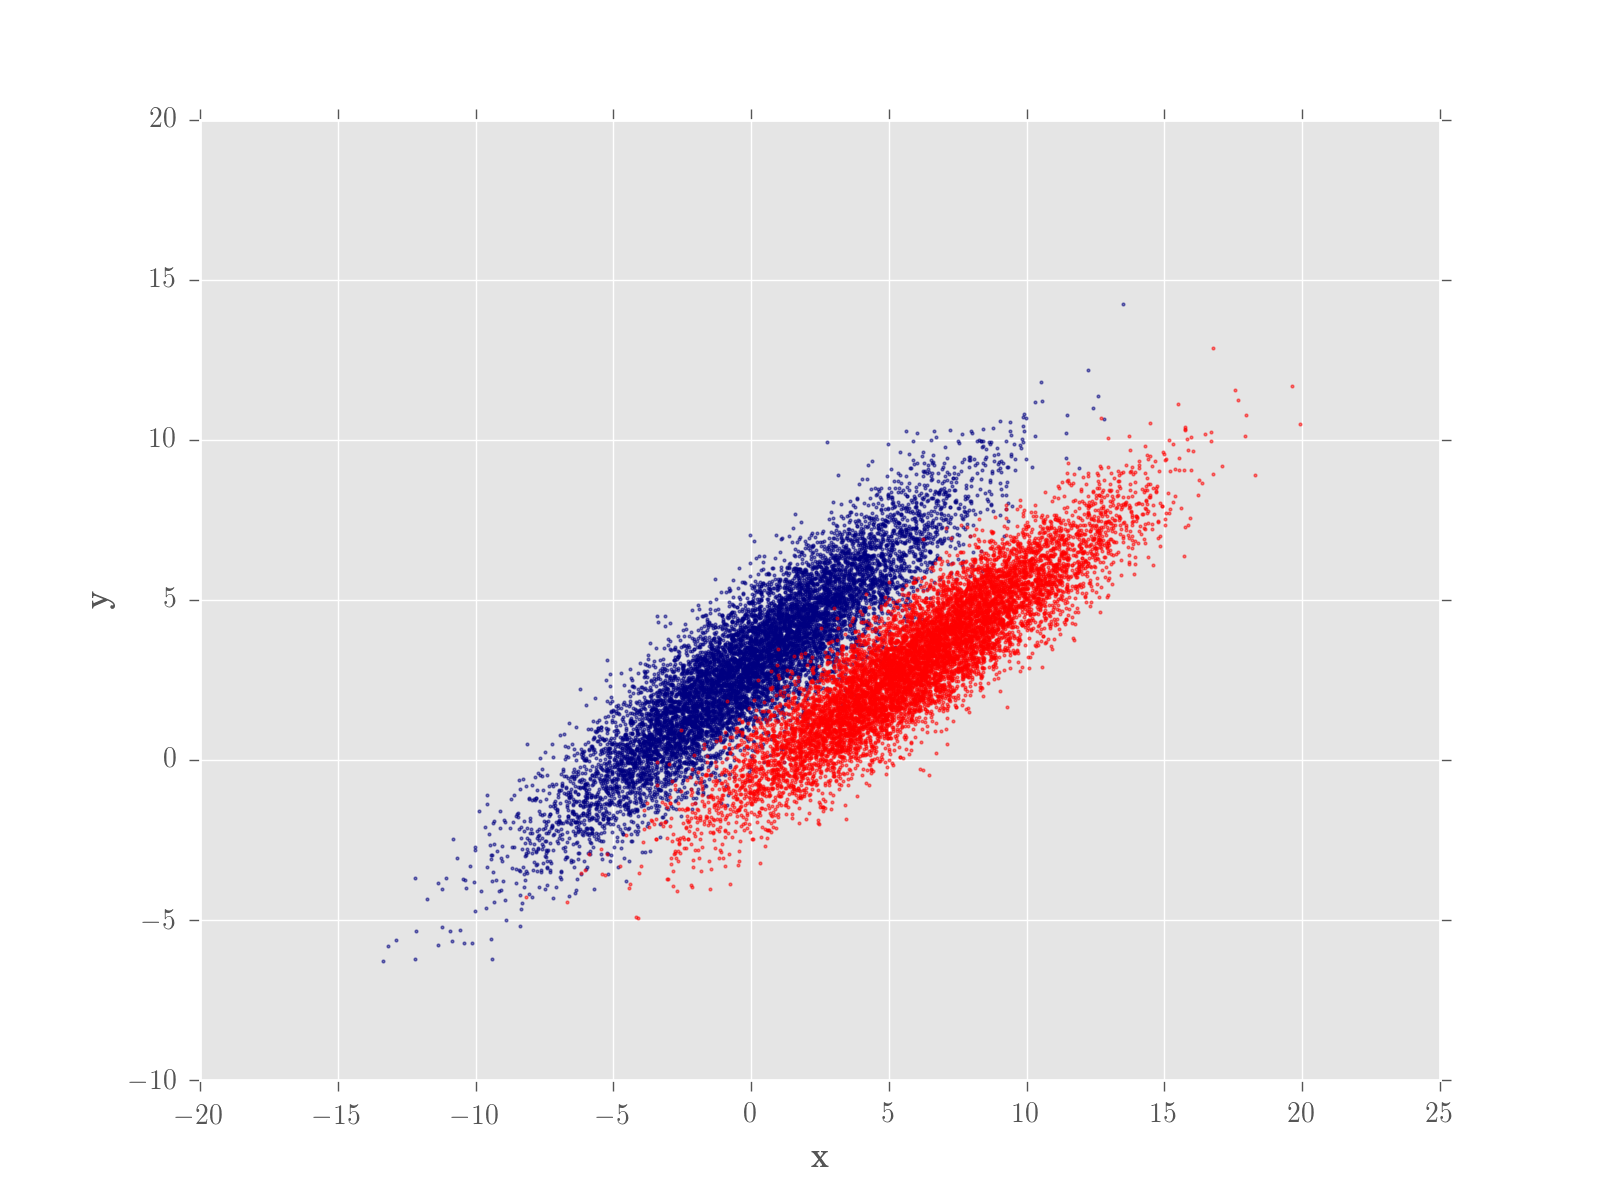
\includegraphics[width=0.7\textwidth]{1b.png}
	\caption{Zweidimensionaler Scatterplot der Populationen.}
\end{figure}
\begin{itemize}
\item[c)]
Die Stichprobenmittelwerte sind $x_{\text{mean}} = 6.026$ und $y_{\text{mean}} = 3.125$,
Die Varianzen sind $var_x = 12.225$ und $var_y = 5.365$.
Die Kovarianz ist $cov_xy = 7.321$ und der Korellationskoeffizient $\rho_{xy} = 0.904$
\end{itemize}


\section*{Aufgabe 2: \emph{Trennende Geraden}}

\begin{figure}
	\centering
	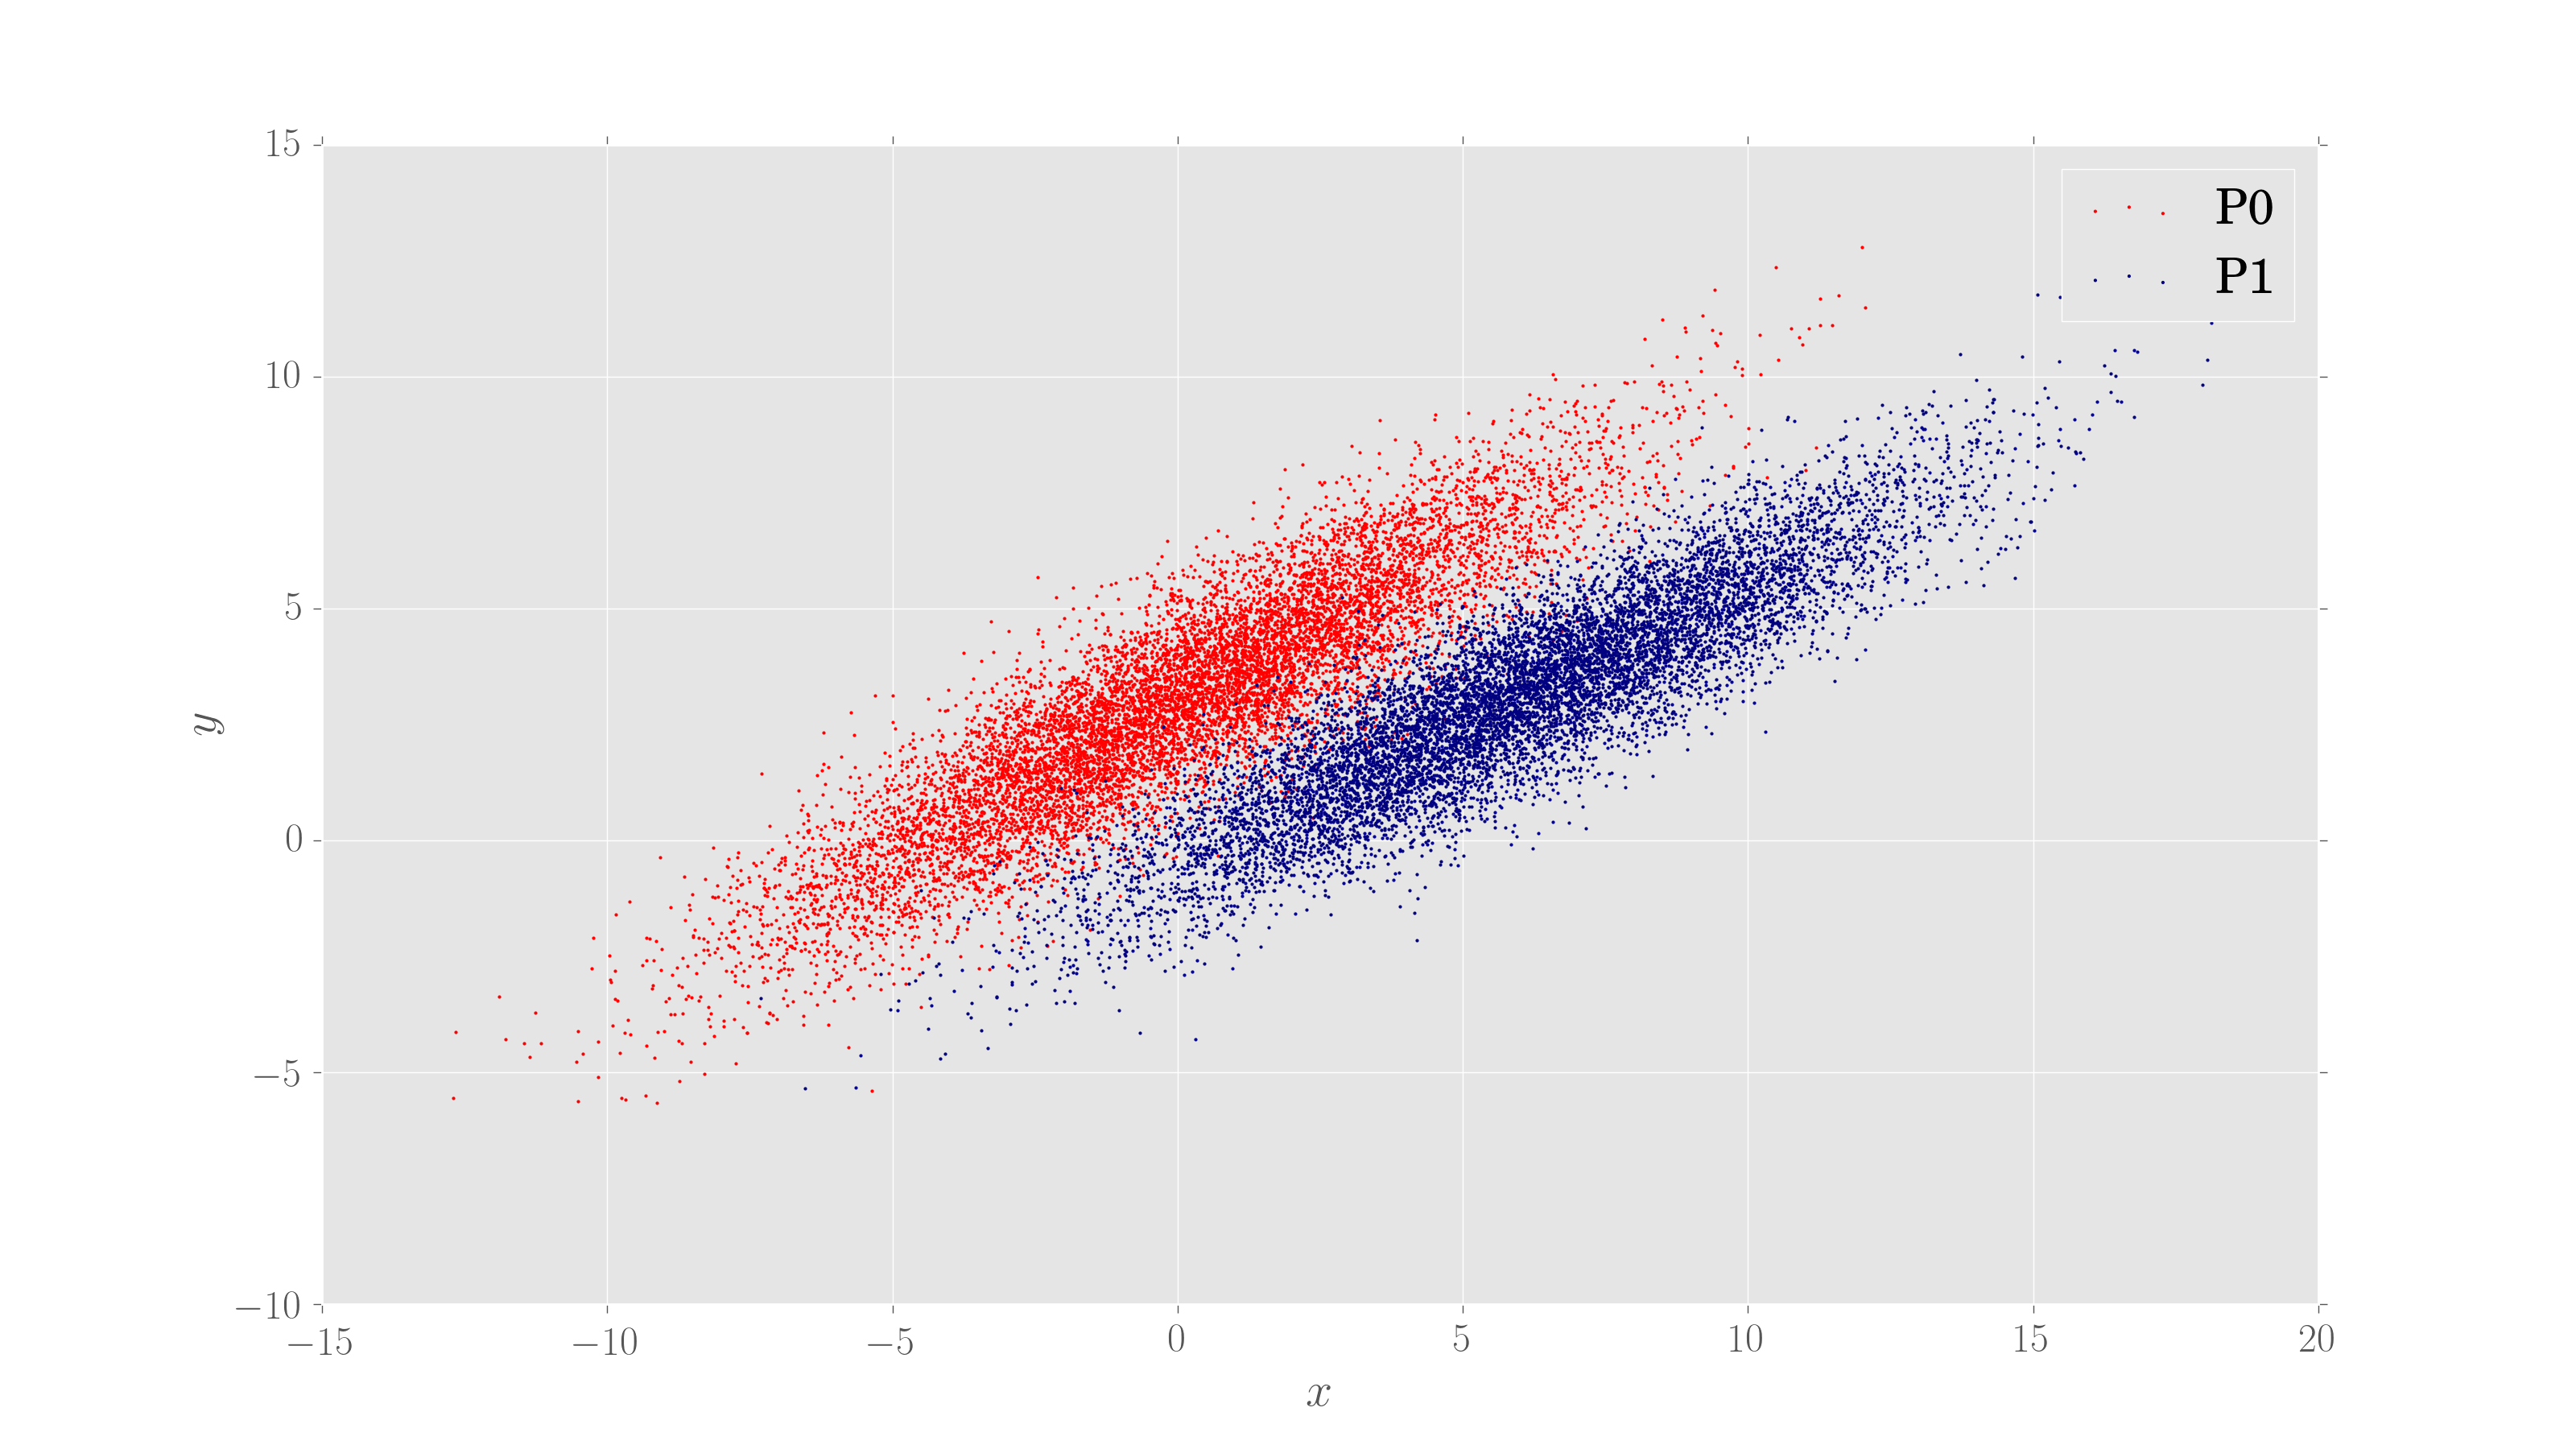
\includegraphics[width=0.7\textwidth]{scatter_P0_P1.png}
	\caption{Zweidimensionaler Scatterplot der Populationen.}
\end{figure}
\begin{figure}
	\centering
	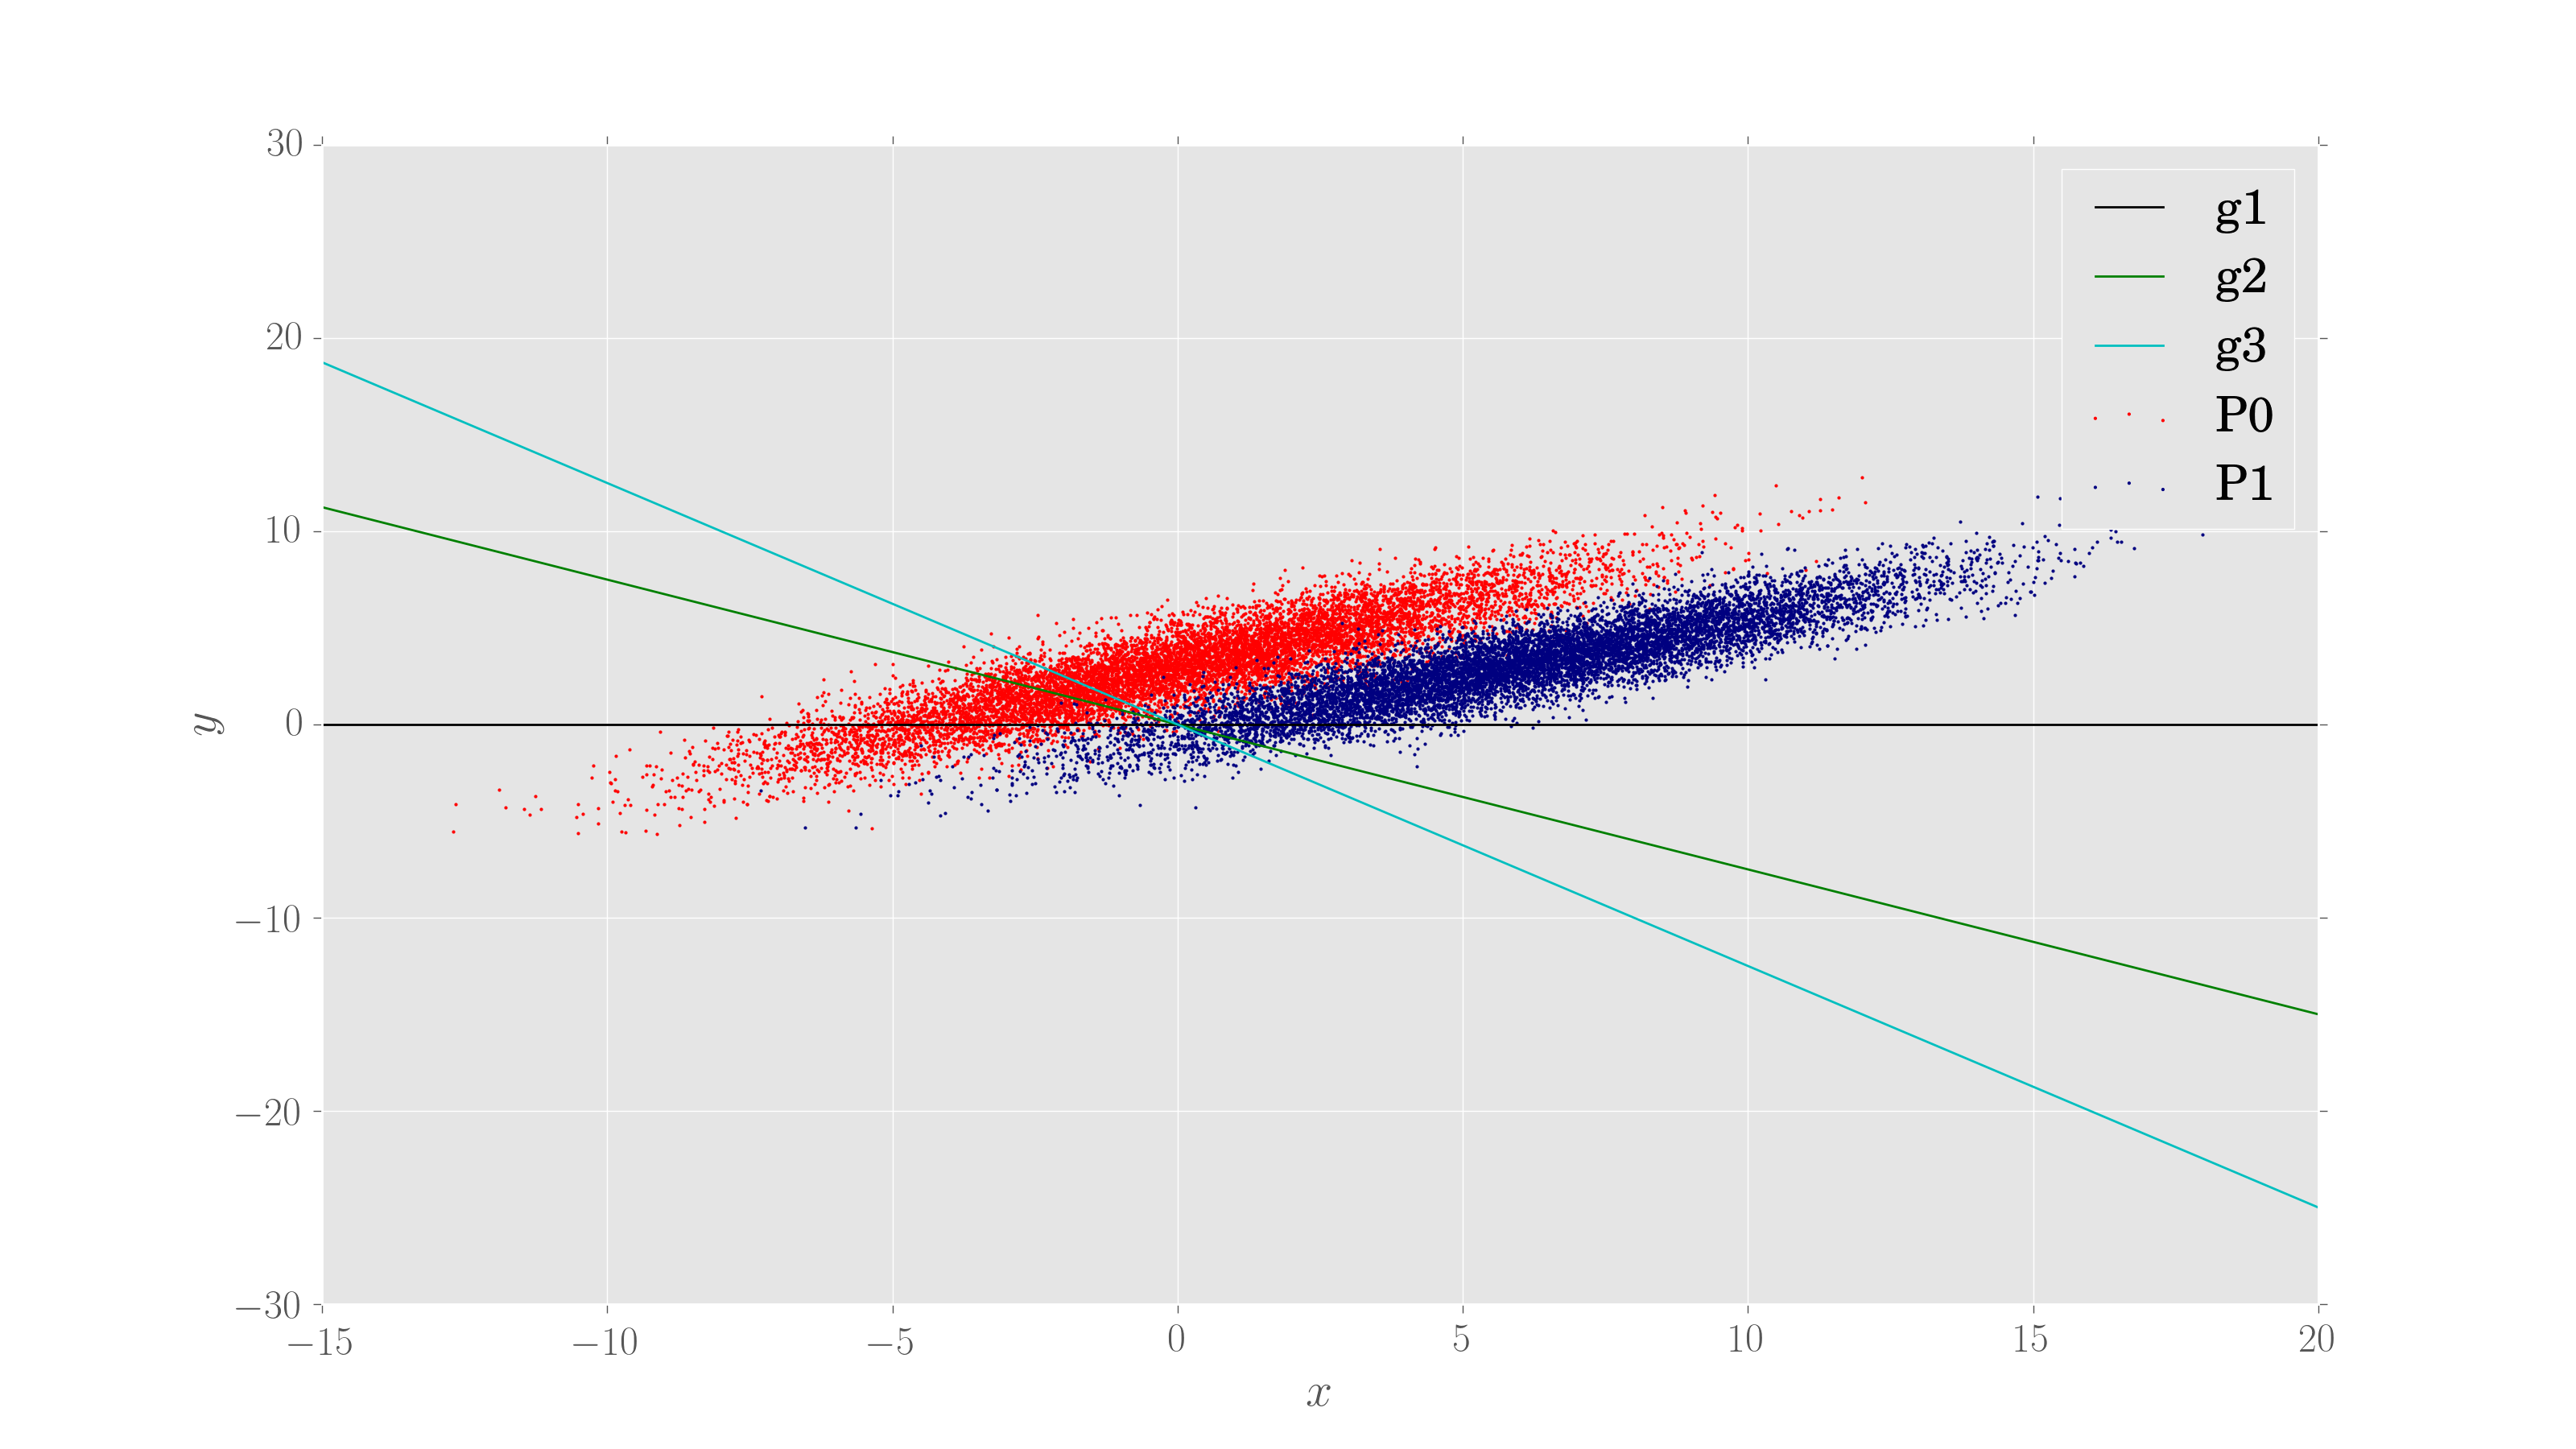
\includegraphics[width=0.7\textwidth]{scatter_with_lines.png}
	\caption{Zweidimensionaler Scatterplot der Populationen mit eingezeichneten Projektionsgeraden.}
\end{figure}
\begin{figure}
	\centering
	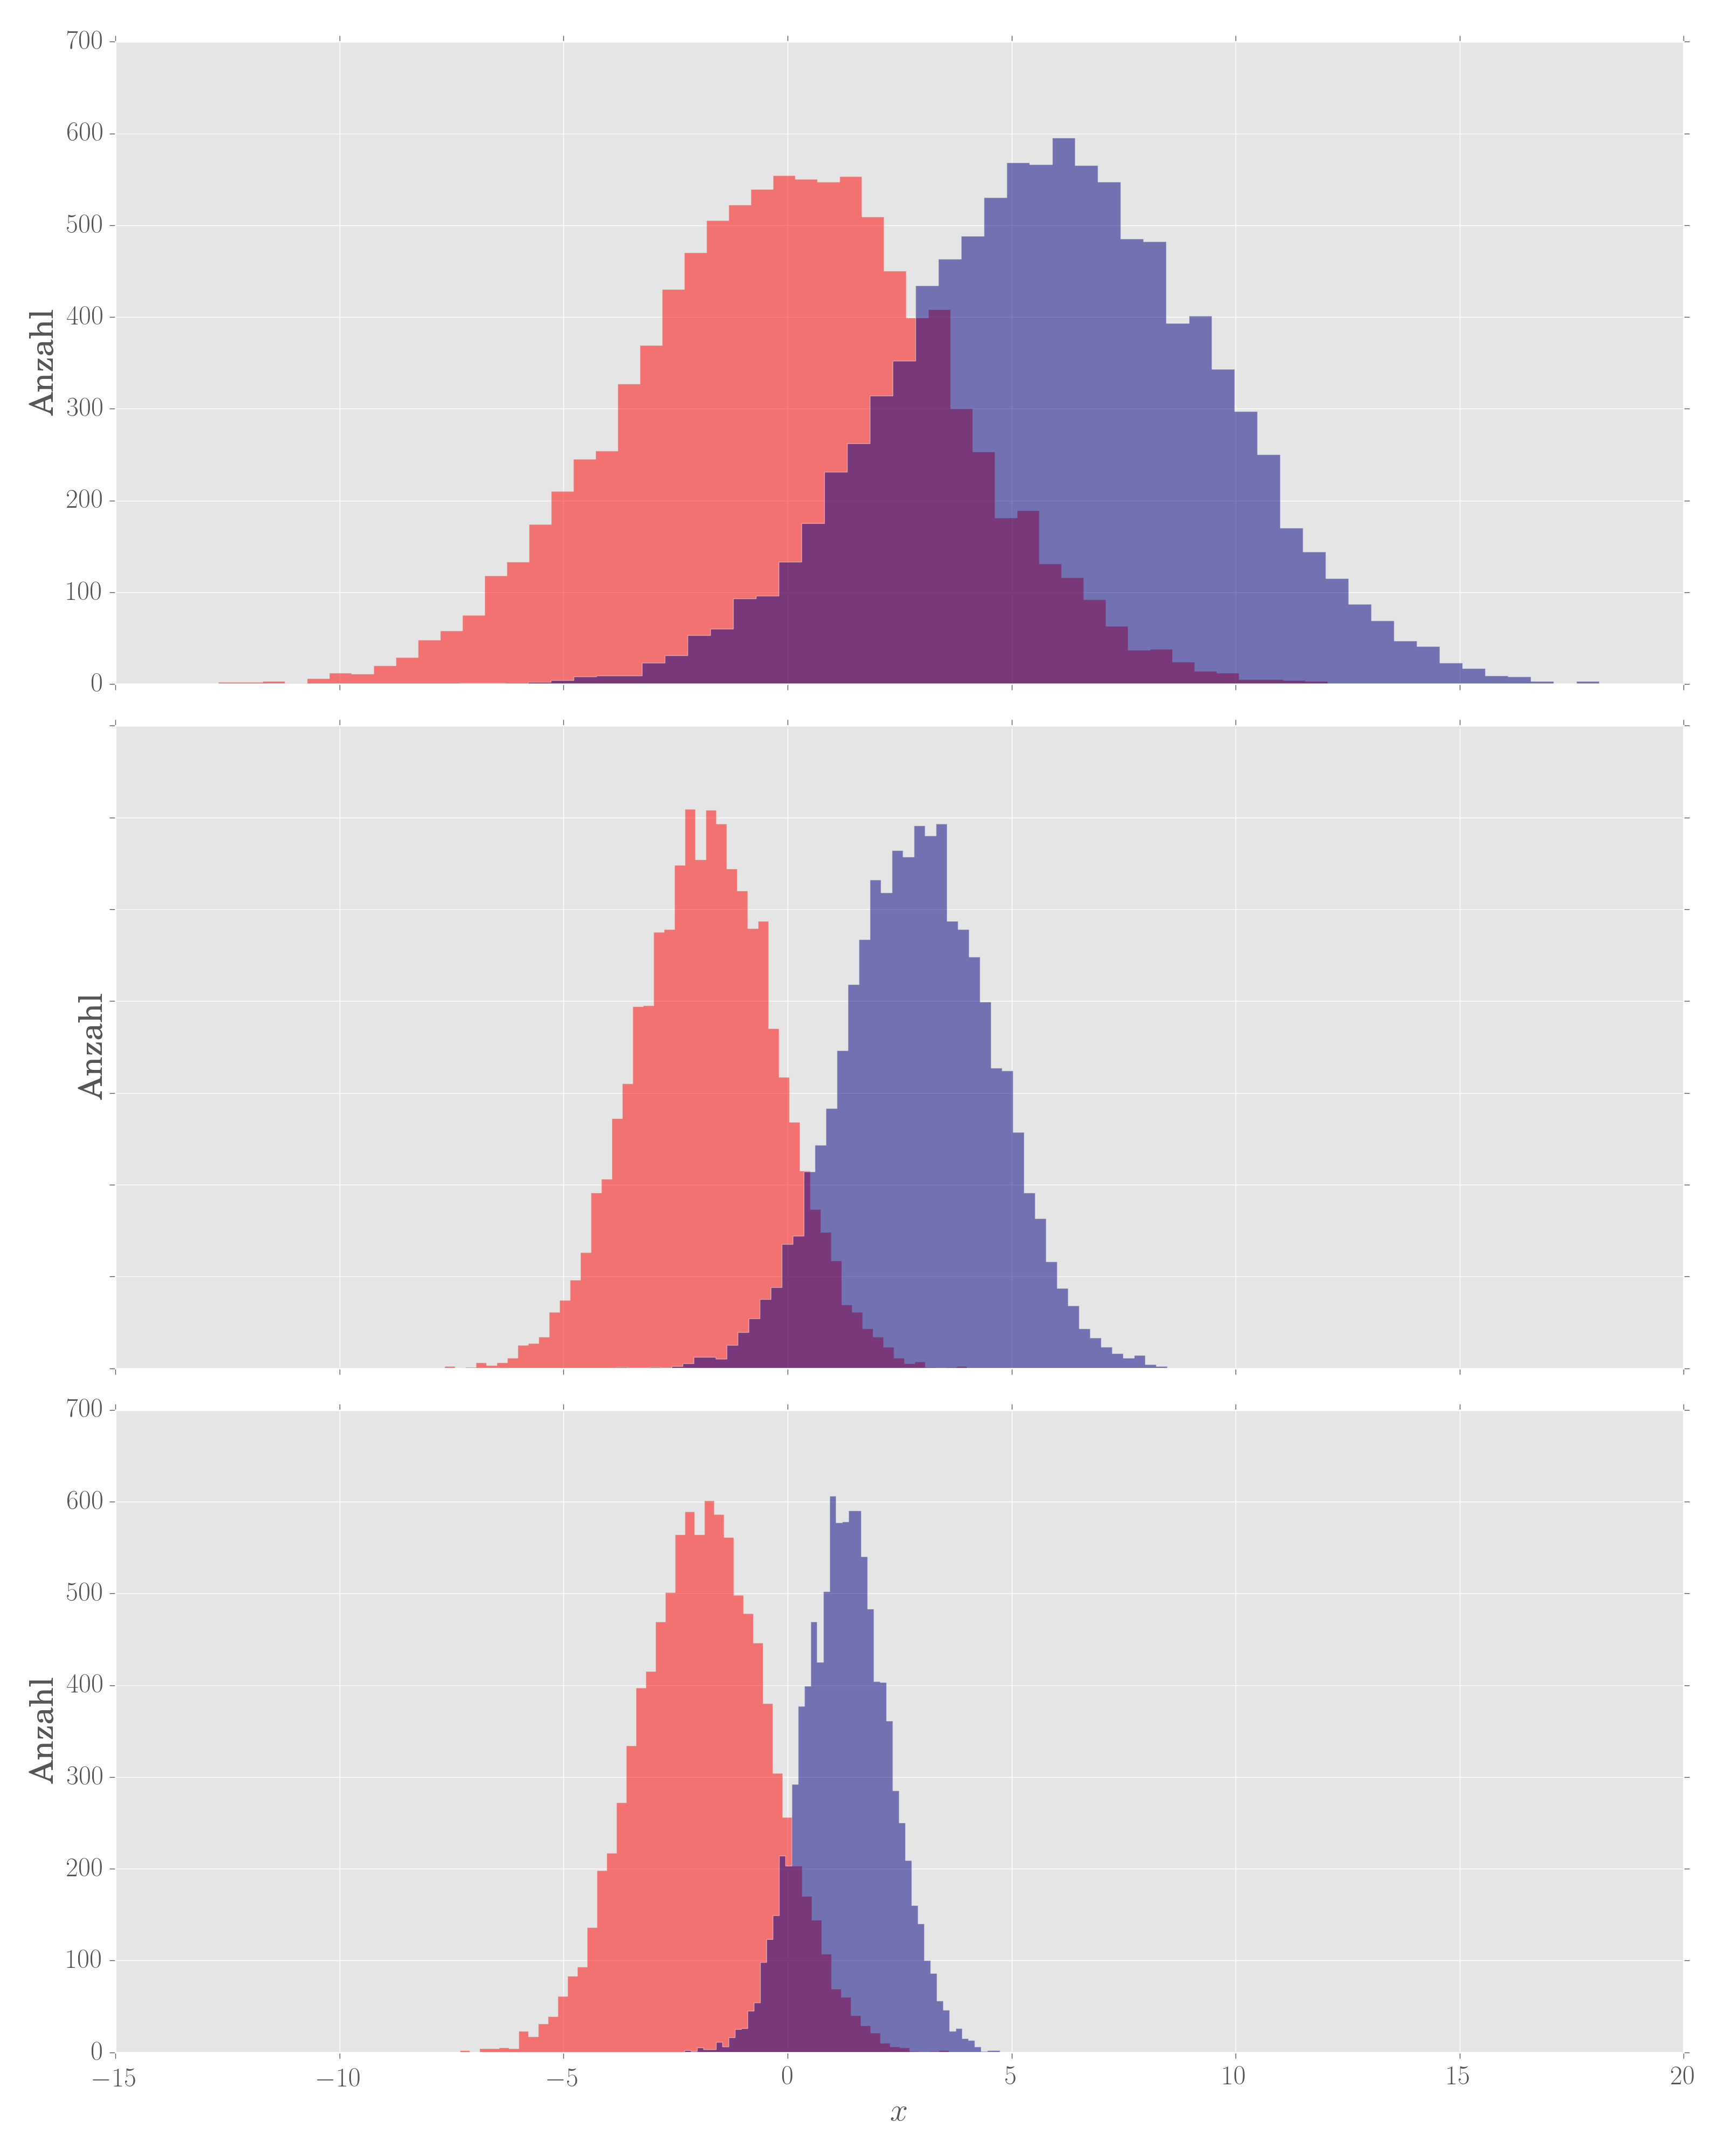
\includegraphics[width=0.7\textwidth]{hists_proj.png}
	\caption{Projektion der Populationen auf die Geraden $g_1$,$g_2$ und $g_3$}
\end{figure}

\begin{figure}
	\centering
	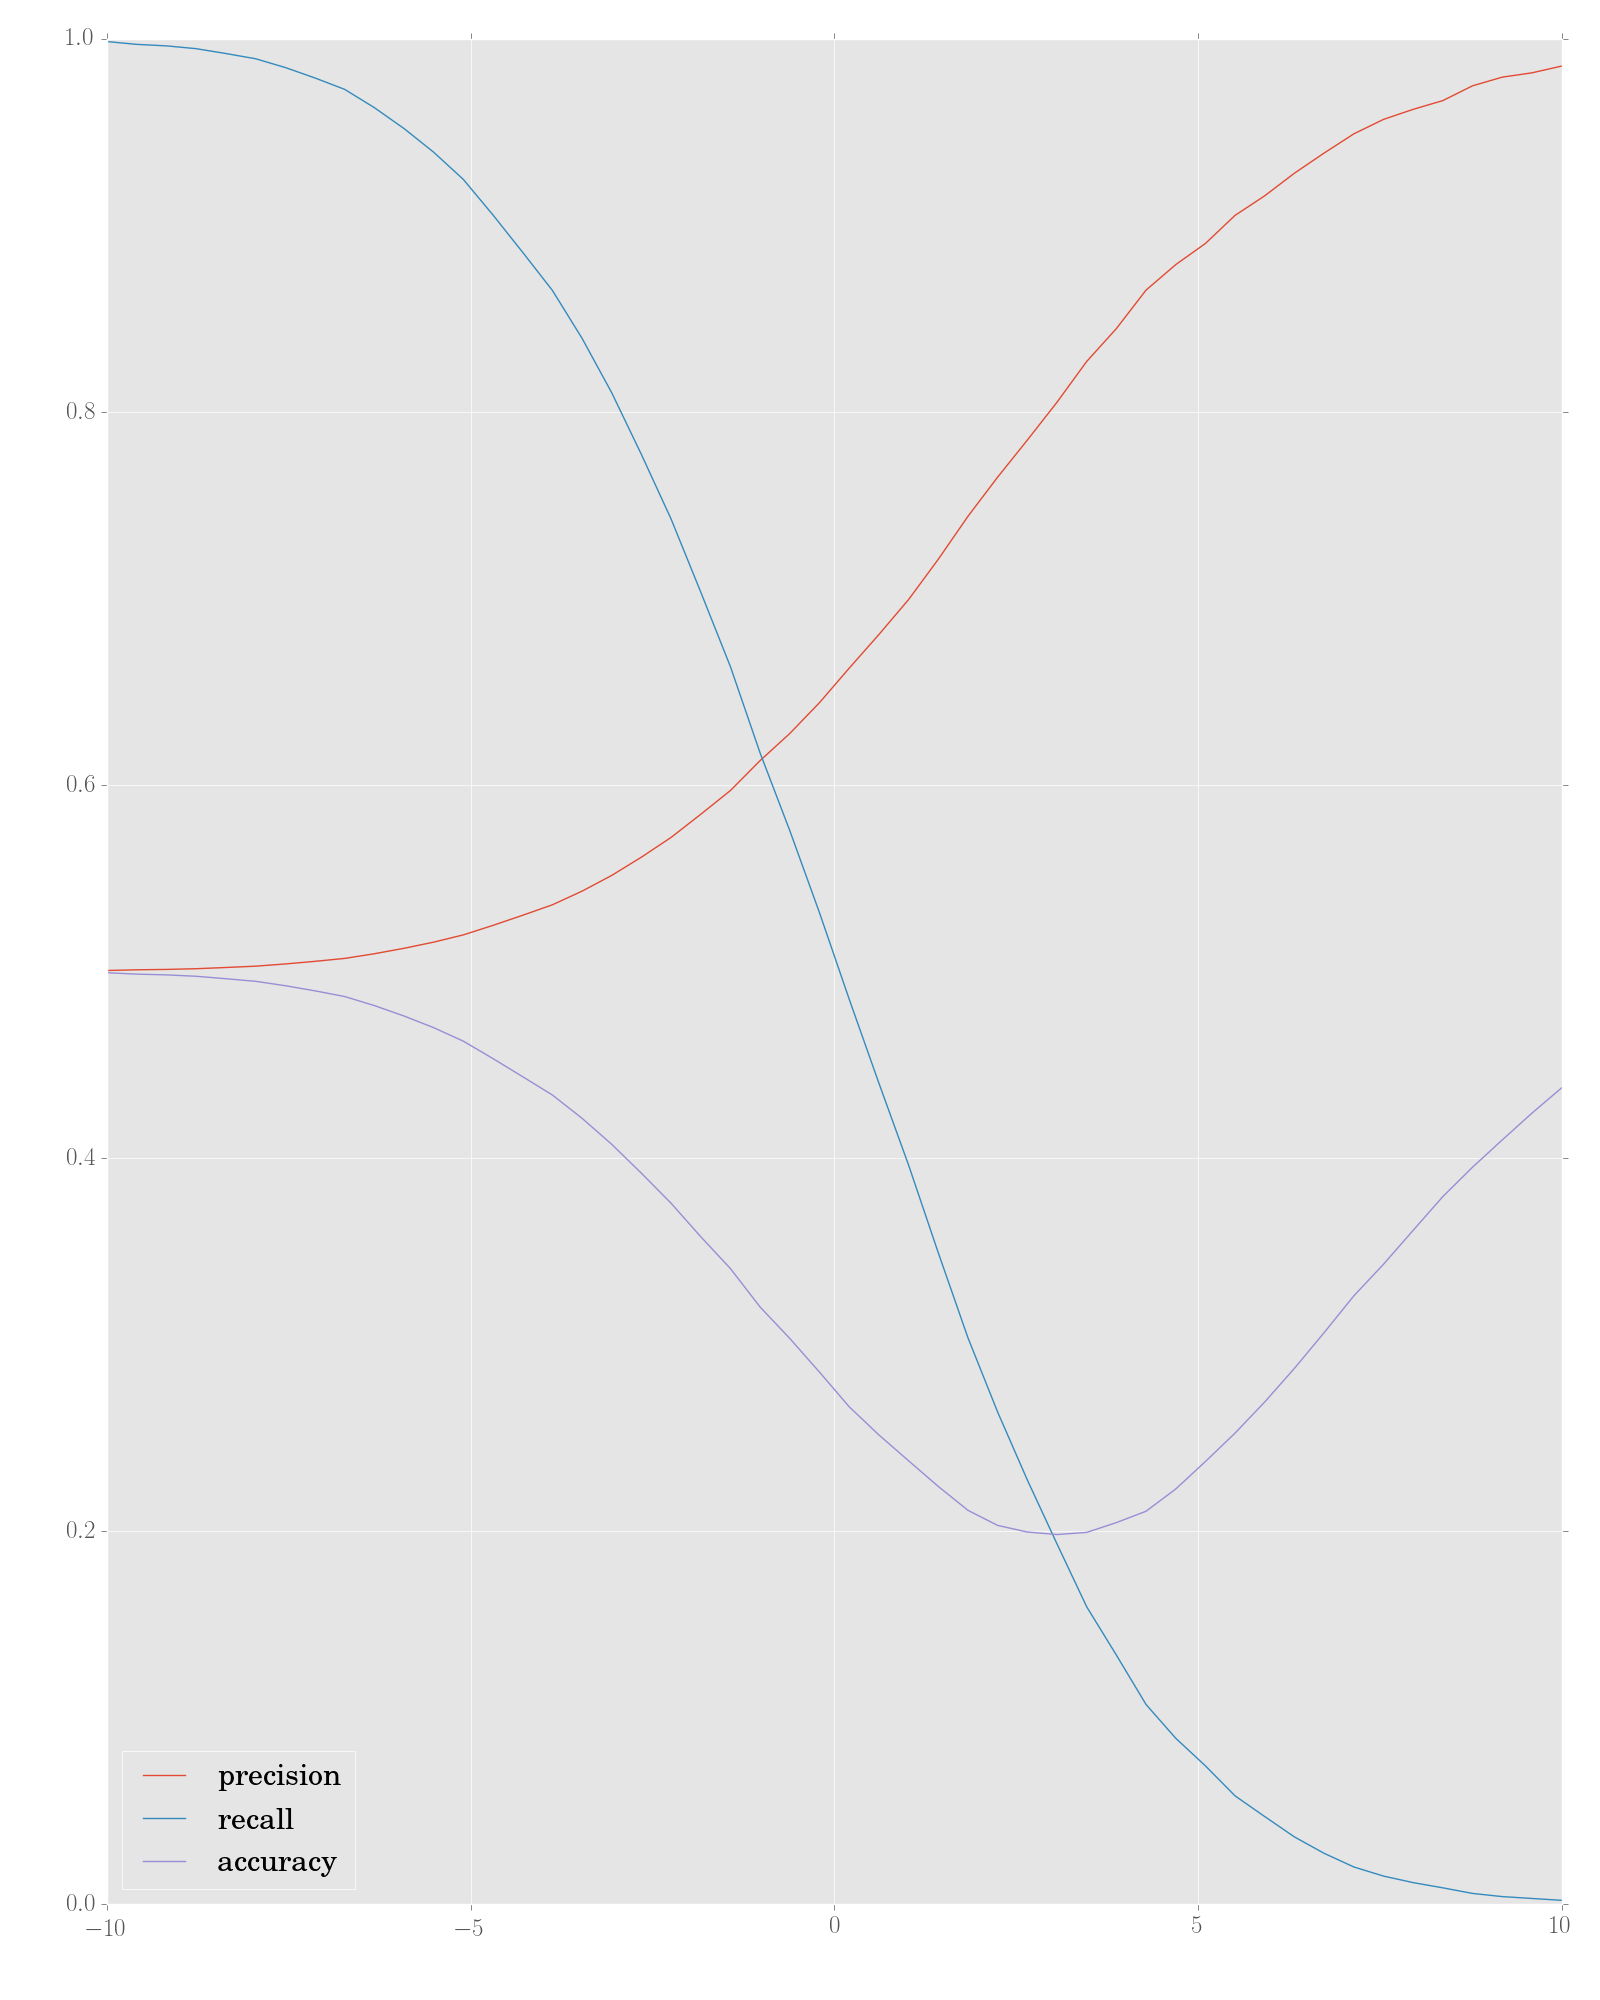
\includegraphics[width=0.7\textwidth]{performace_g1.png}
	\caption{Reinheit (precision), Effizienz (accuracy) und Sensitivität (recall) für die Gerade $g_1$}
\end{figure}
\begin{figure}
	\centering
	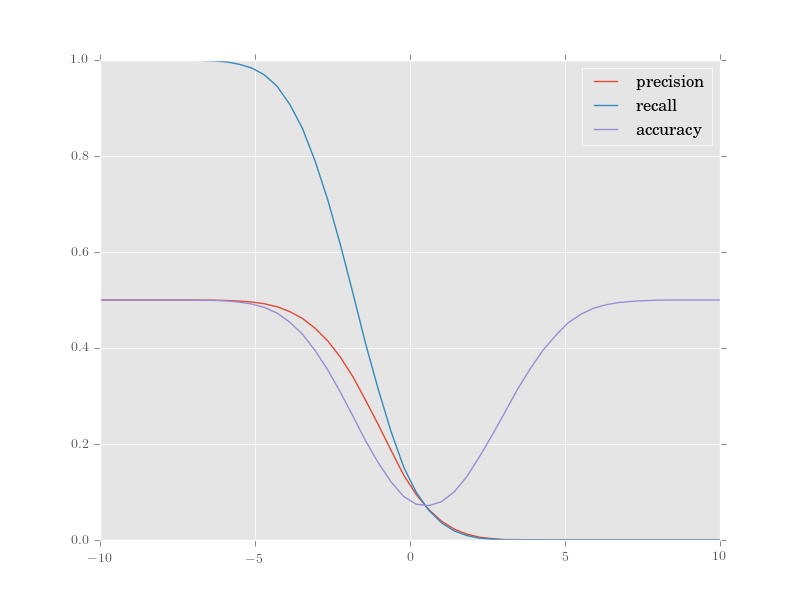
\includegraphics[width=0.7\textwidth]{performace_g2.png}
	\caption{Reinheit (precision), Effizienz (accuracy) und Sensitivität (recall) für die Gerade $g_2$}
\end{figure}

\begin{figure}
	\centering
	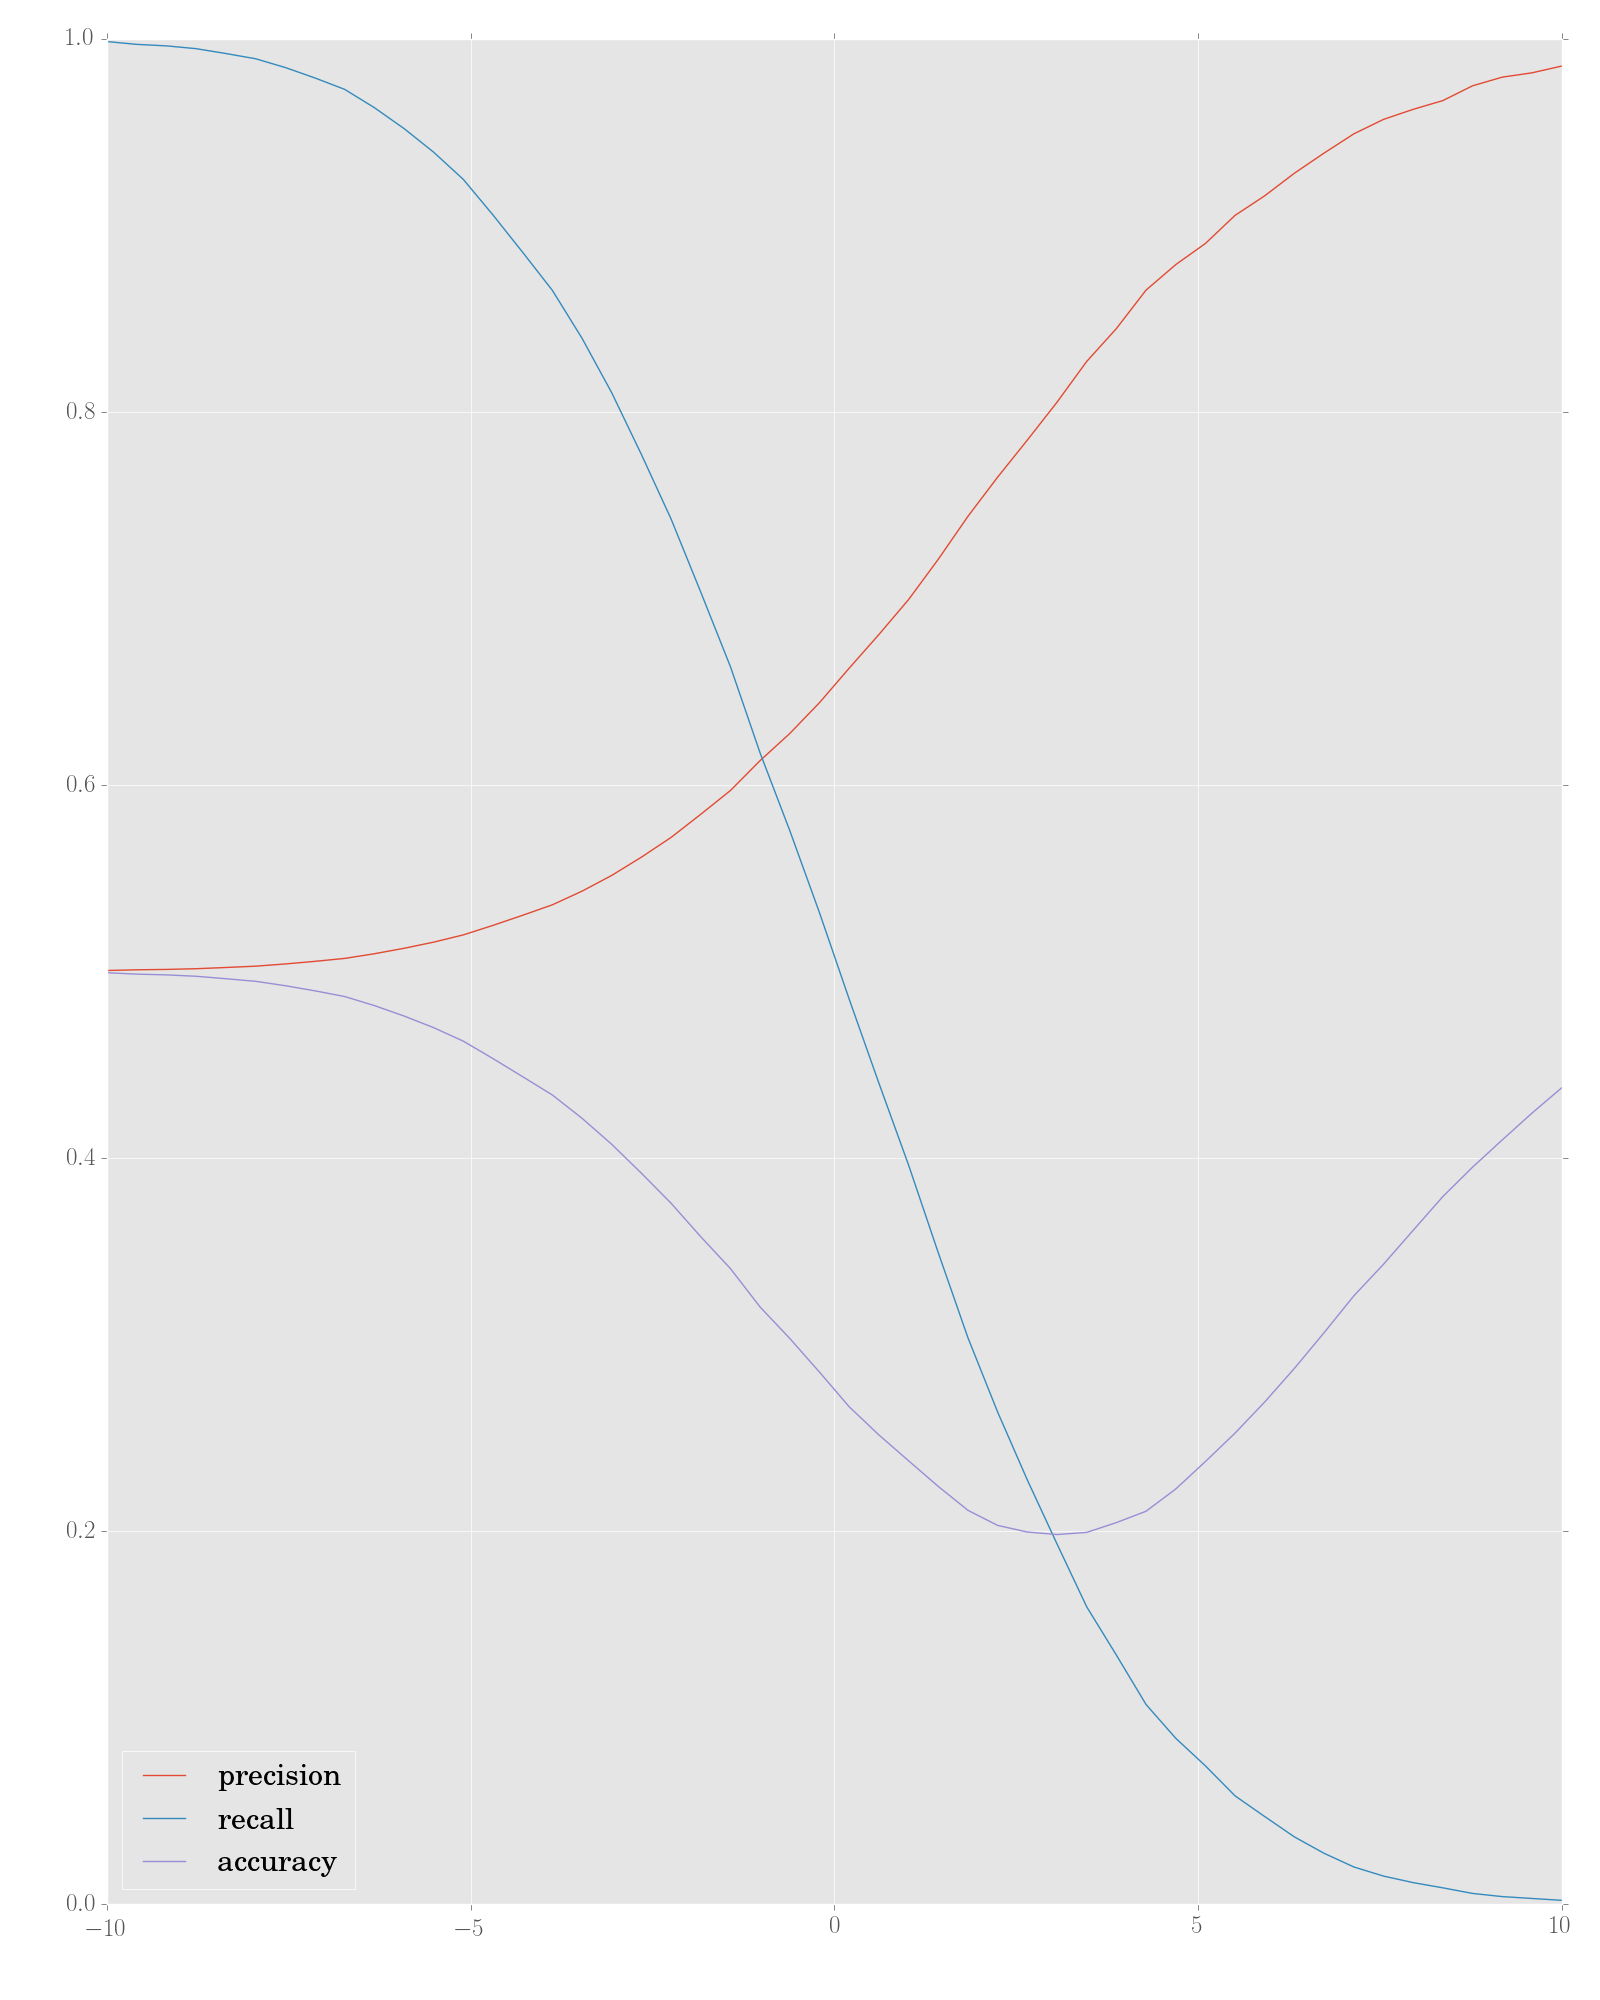
\includegraphics[width=0.7\textwidth]{performace_g1.png}
	\caption{Reinheit (precision), Effizienz (accuracy) und Sensitivität (recall) für die Gerade $g_3$}
\end{figure}



\section*{Aufgabe 3: \emph{Fisher--Diskrimanante: Per Hand}}

\section*{Aufgabe 4: \emph{Datenaufbereitung}}

\begin{itemize}

\item[1] Tokenizierung: Zerlegen eines Fließtextes in Tokens (kleine Einheiten) und anschließendes Löschen unbrauchbarer Tokens
\item[Bsp.:] Erstellung von Bbliotheken zu Natural Language Processing
\item[2] Typ und Formatierung einzelner Einträge aneinander anpassen.
\item[Bsp.:] Gleiche Formatierung für Einträge von Daten oder Zeiten.
\item[3] Ersetzen nicht eindeutiger Daten.
\item[Bsp.:] Lücken, NaNs, $\infty$ sinnvoll ersetzen oder löschen.
\item[4] Ersetzen von missverständlichen Informationen.
\item[Bsp.:] Konstanten und fehlende Werte löschen.

\item[b] Eine Normierung sorgt für eine bessere Vergleichbarkeit von Daten.
\item[c] Löschen oder ersetzen von Daten.
\item[d] Daten müssen miteinander kombiniert werden können. Zum Beispiel anpassen von Tabellenlängen beim Zusammenführen, gleiche Formatierung von Daten.
\end{itemize}